\documentclass[12pt]{article}
\usepackage[utf8]{inputenc}
\usepackage[cm]{fullpage}
\usepackage{amssymb}
\usepackage{multicol}
\usepackage{graphicx}

\newcommand{\exerc}[3]{ \vspace*{25pt} {$\mathbf{#1)}$} #2 \hfill {\it #3} }
\newcommand{\exitem}[2]{ \texttt{\bf #1)} #2 \\ }
\newcommand*\xor{\mathbin{\oplus}}
\renewcommand{\neg}[1]{ 
  \mkern 1.5mu\overline{\mkern-1.5mu#1\mkern-1.5mu}\mkern 1.5mu
}

\newenvironment{exitems}[1]{
\\
\hspace*{30pt}
\begin{minipage}{0.8\textwidth}
\begin{multicols}{#1} 
}{
\end{multicols}
\end{minipage}
}

\newenvironment{exitemss}[1]{
\\
\hspace*{30pt}
\begin{minipage}{0.8\textwidth}
#1
}{
\end{minipage}
}

\begin{document}

\pagenumbering{gobble}

\begin{center}
{\Large \bf Elementos de Lógica Digital - 2015/2}
\end{center}

{\large \bf Prova Final}

{\bf Professor:} Marcos Daniel Baroni

{\bf Data:} 10/12/2015

\exerc{1}{Simplifique as expressão abaixo utilizando álgebra de Boole.}{(2.5 pontos)}
\\ \hspace*{3em} \exitem{a}{
     $S = \neg{(\neg{A}B + C\neg{D} + AD)}+\neg{A}$
   }
   \hspace*{3em} \exitem{b}{
      $S = [\neg{ (\neg{\neg{B} + \neg{D}})\neg{(B + C)}+ C}] + \neg{A}\neg{B}C + \neg{B}(\neg{A+C})$
   }

\exerc{2}{Implemente a tabela verdade de circuito contenha uma entrada $X$ que
  funcione como um somador completo quando $X=0$ e como um subtrator completo quando $X=1$.}{(2.5 pontos)}
\begin{center}
  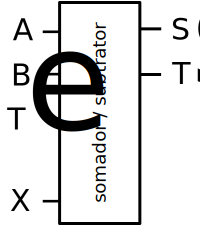
\includegraphics[scale=0.5]{circ}
\end{center}

\exerc{3}{Projete um contador síncrono que execute a sequência abaixo.}{(2.5 pontos)}
\begin{center}
  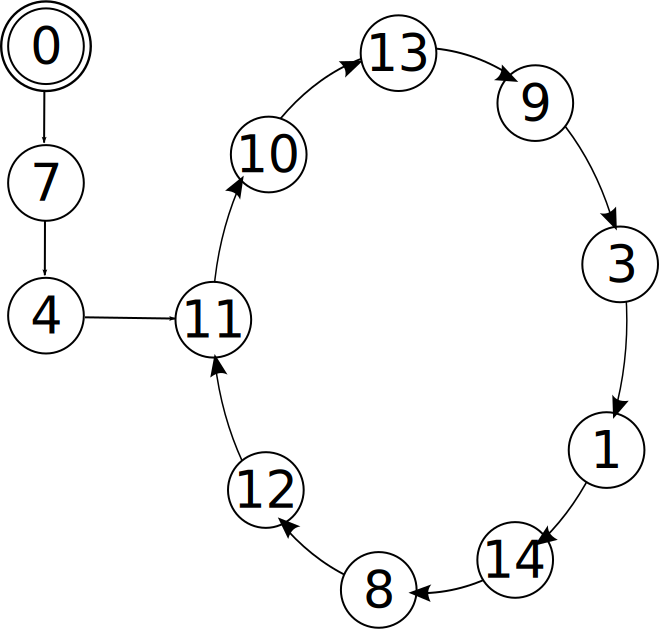
\includegraphics[scale=0.25]{seq}
\end{center}

\exerc{4}{Utilizando blocos RAM 64x4, esquematize uma RAM 64x8 e especifique as
  características abaixo sobre a memória resultante.}{(2.5 pontos)}
\\
\begin{center}
\begin{tabular}{|l|c|c|}
 \cline{2-2}
 \multicolumn{1}{c|}{} & {\bf RAM 64x8} \\ \hline
 Capacidade total & \phantom{aaaaaaaaaaaaaa} \\ \hline
 Largura de palavra de dados & \\ \hline
 Largura da barra de endereços & \\ \hline
 Palavra de endereço inicial (em hexadecimal) & \\ \hline
 Palavra de endereço final (em hexadecimal) & \\ \hline
\end{tabular}
\end{center}

\end{document}

